\documentclass[10pt]{article}
\usepackage[top=1in,left=1.75in,footskip=0.75in]{geometry}

% amsmath and amssymb packages, useful for mathematical formulas and symbols
\usepackage{amsmath,amssymb}
\usepackage{pifont}
% \usepackage{titling}
\usepackage{blindtext}
\usepackage{tablefootnote}
\usepackage{authblk}
\usepackage{array}
\newcolumntype{L}[1]{>{\raggedright\let\newline\\\arraybackslash\hspace{0pt}}m{#1}}
\newcolumntype{C}[1]{>{\centering\let\newline\\\arraybackslash\hspace{0pt}}m{#1}}
\newcolumntype{R}[1]{>{\raggedleft\let\newline\\\arraybackslash\hspace{0pt}}m{#1}}


% \usepackage{changepage} % Use adjustwidth environment to exceed column width (see example table in text)
\usepackage[utf8x]{inputenc} % Use Unicode characters when possible
\usepackage{textcomp,marvosym} % textcomp package and marvosym package for additional characters
\usepackage{cite} % cite package, to clean up citations in the main text. Do not remove.
\usepackage{nameref,hyperref} % Use nameref to cite supporting information files (see Supporting Information section for more info)
\usepackage[right]{lineno} % line numbers
\usepackage{microtype} % ligatures disabled
\DisableLigatures[f]{encoding = *, family = * }
\usepackage{epstopdf}

% color can be used to apply background shading to table cells only
\usepackage[table]{xcolor}

% array package and thick rules for tables
\usepackage{array}

% bold math symbols package
\usepackage{bm}

% nice figures and captions
\usepackage{graphicx}

%\renewcommand{\arraystretch}{1.2}
%\setlength{\tabcolsep}{12pt}

% create "+" rule type for thick vertical lines
\newcolumntype{+}{!{\vrule width 2pt}}

% create \thickcline for thick horizontal lines of variable length
% \newlength\savedwidth
% \newcommand\thickcline[1]{%
%   \noalign{\global\savedwidth\arrayrulewidth\global\arrayrulewidth 2pt}%
%   \cline{#1}%
%   \noalign{\vskip\arrayrulewidth}%
%   \noalign{\global\arrayrulewidth\savedwidth}%
% }
% \thickhline command for thick horizontal lines that span the table
% \newcommand\thickhline{\noalign{\global\savedwidth\arrayrulewidth\global\arrayrulewidth 2pt}%
% \hline
% \noalign{\global\arrayrulewidth\savedwidth}}
% Remove comment for double spacing
%\usepackage{setspace} 
%\doublespacing
% Text layout
\raggedright
\setlength{\parindent}{0.5cm}
\textwidth 5.25in 
\textheight 8.75in

% Bold the 'Figure #' in the caption and separate it from the title/caption with a period
% Captions will be left justified
\usepackage[aboveskip=1pt,labelfont=bf,labelsep=period,justification=raggedright,singlelinecheck=off]{caption}
\renewcommand{\figurename}{Fig}

% Use the PLoS provided BiBTeX style
%\bibliographystyle{plos2015}

% Remove brackets from numbering in List of References
\makeatletter
\renewcommand{\@biblabel}[1]{\quad#1.}
\makeatother

% Header and Footer with logo
% \usepackage{lastpage,fancyhdr,graphicx}

%\pagestyle{myheadings}
% \pagestyle{fancy}
% \fancyhf{}
% \rfoot{\thepage/\pageref{LastPage}}
% \renewcommand{\headrulewidth}{0pt}
% \renewcommand{\footrule}{\hrule height 2pt \vspace{2mm}}
% \fancyheadoffset[L]{2.25in}
% \fancyfootoffset[L]{2.25in}
%\lfoot{\today}

%% Include all macros below

\newcommand{\lorem}{{\bf LOREM}}
\newcommand{\ipsum}{{\bf IPSUM}}

%% END MACROS SECTION

% Insert author names, affiliations and corresponding author email (do not include titles, positions, or degrees).
\title{Nearest-neighbor Projected-Distance Regression (NPDR) detects network interactions and controls for confounding and multiple testing} 
\author[1]{Trang T. Le}
\author[2]{Bryan A. Dawkins}
\author[2,3*]{Brett A. McKinney}
\affil[1]{Department of Biostatistics, Epidemiology and Informatics,
University of Pennsylvania, Philadelphia, PA 19104}
\affil[2]{Department of Mathematics, University of Tulsa, Tulsa, OK 74104}
\affil[3]{Tandy School of Computer Science, University of Tulsa, Tulsa, OK 74104}
\renewcommand{\Authands}{ and }
\date{\today}


\usepackage{Sweave}
\begin{document}
\Sconcordance{concordance:main_npdr.tex:main_npdr.Rnw:%
1 111 1 1 0 493 1}

\setkeys{Gin}{width=1\textwidth}
% \begin{titlingpage}
\maketitle
\begin{abstract}
        
We develop a new feature selection technique that uses the generalized linear model (GLM) to perform regression between nearest-neighbor pair distances projected onto attributes to address a broad spectrum of statistical challenges in high-dimensional data, including interactions and confounding variables.
Recently we developed STatistical Inference Relief (STIR), a pseudo t-test approach to estimate the statistical significance of Relief-based attribute scores for binary outcome (classification) problems, where the data may involve main effects and complex statistical interactions (network epistasis).
However, efficient statistical inference methods are needed to detect complex network effects in more complicated modeling situations, including continuous outcomes, mixtures of categorical and continuous predictors, and correcting for potential confounding variables.
Our new Nearest-neighbors Projected-Distance Regression (NPDR) encompasses STIR for binary outcome data and extends its capabilities to statistically correct for covariates, which previously was not feasible for Relief-based methods.
NPDR provides a novel and improved way to compute regression-based Relief scores (RRelief) for quantitative outcomes that also allows statistical corrections and various combinations of predictor data types such as genetic variants and gene expression.
In addition, we implement a penalized version of NPDR and derive the theoretical constant-$k$ approximation to the expected number of neighbors for spatially uniform radial neighborhoods. 
%novel and broad formalism using the generalized linear model that allows for the calculation of Relief-based statistical significance for classification and regression problems along with the ability to correct for confounding factors.  
Using realistic simulations that include main effects and gene-network interactions, we show for that NPDR improves attribute estimates compared to standard Relief while also being able to compute statistical significance of attributes and adjust for covariates.
We demonstrate that the NPDR framework has similar statistical properties to the pseudo t-test based method for binary outcome data with the added flexibility of regression modeling. We also compare glmnet with the penalized version of NPDR.
We use RNA-Seq data from a study of major depressive disorder to show that NPDR with covariate adjustment removes spurious associations due to confounding by sex. 
\\
% \textbf{Availability:} Code and data available at {{https://insilico.github.io/npdr/}}.\\
% \textbf{Contact:} {{brett.mckinney@gmail.com}}\\
% \textbf{Supplementary information:} Supplementary data are available online.

\end{abstract}
% \end{titlingpage}

\linenumbers

\section{Introduction}

Relief-based algorithms are efficient nearest-neighbor feature selection methods that are able to detect epistasis or statistical interaction effects in high-dimensional data without resorting to pairwise modeling of attributes \cite{urbanowicz17b,kononenko97, mckinney09, rendell92}. Epistasis is a measure of the effect of mutations on a phenotype beyond what would be expected by their independent effects. There is evidence that these non-independent effects are pervasive~\cite{breen12} and that higher-order interactions also play an important role in genetics~\cite{weinreich13}. 

A similar effect can be observed in differential co-expression, where the phenotypic effect of one gene is modified depending on the expression of another gene \cite{lareau15,diffcoexp10}. The embedding of these interactions in a regulatory network may lead to, not only pairwise interactions, but also higher-order epistasis network effects. Attempting to model these higher order interactions combinatorially would be computationally and statistically intractable~\cite{riesselman18}. Thus, computationally scalable feature selection methods, like Relief, are needed to capture these higher-order effects in high-dimensional data such as genome-wide association~\cite{titv} and gene expression studies~\cite{stir}.

We recently introduced the STatistical Inference Relief (STIR) formalism~\cite{stir} to address Relief-based methods' lack of a statistical distribution for hypothesis testing and the challenge of assessing the false positive rate of Relief-based scores.
STIR extended Relief-based methods to compute statistical significance of attributes in binary outcome data (e.g. case-control) by reformulating the Relief weight~\cite{mckinney13} as a pseudo t-test for the difference of means between neighbors with the same and opposite phenotype (hits and misses).
The STIR group means are computed from the difference of projected-distance differences between neighbors onto a given attribute dimension. We showed that STIR is an effective approach with high power and low false-positive rates for data with main and interaction effects. 
STIR is applicable to any predictor data type (numeric/expression or categorical/SNP); however, being based on a t-test, it does not apply to data with continuous outcome (e.g., quantitative trait) and does not correct for covariates.
Prior to the current study, no Relief-based method includes covariate correction.  

In the current study, we extend STIR to projected distance-based regressions with the generalized linear model (GLM).
This new Nearest-neighbors Projected-Distance Regression (NPDR) approach opens up Relief-based methods to statistical inference for a broad class of problems by treating the pairwise projected-distance differences among nearest neighbors as the observations in a GLM.
The projected difference function between two instances for a given attribute may be simply an arithmetic difference for numeric attributes or may be tailored to the specific data type, such as genetic variants~\cite{titv}.
The NPDR formalism encompasses binary outcome (classification) problems (Eq.~\ref{eq:too_logit}), leads to a new and seamless way of solving numeric outcome (regression) problems (Eq.~\ref{eq:lin_reg}) and adjusts for covariates (Eq.~\ref{eq:lin_reg_cov}) while detecting main effects and interactions. 

Covariate adjustment is important throughout biomedical research to avoid confounding by demographic variables, like age~\cite{le18_brainagesim} or population stratification~\cite{popstrat16}, but adjusting for covariates is often neglected in machine learning. Relief-based methods also suffer from confounding, but this limitation has not been addressed previously. Some proposed methods for correcting machine learning algorithms include restricted permutation~\cite{rao2017}, inverse probability weighting of training samples~\cite{linn2016} and penalized support vector machines~\cite{li2011ccsvm}. Our NPDR framework leads to a natural way to control for covariates by including additional terms for the between-neighbor projected differences for each covariate within the GLM. We demonstrate the effectiveness of NPDR to correct for confounding on an RNA-Seq study of major depressive disorder in which there is a strong signal in the expression data due to the sex of study participants. 

For each attribute, the NPDR model fits a GLM of projected-distance differences (onto the attribute) between all pairs of nearest-instance neighbors.
For the outcome variable in the model, the projected distances between instances are binary match/mismatches for binary outcome data and arithmetic differences for quantitative outcomes.
The model is linear for regression problems and logistic for binary outcome problems, and either model may include terms for covariates.
The importance of an attribute is given by its [standardized] regression coefficient and the statistical significance by its P value.
The model gives the appearance of being univariate but implicitly accounts for interactions with all other attributes via the neighborhood calculation in the space of all attributes (omnigenic).
NPDR is applicable to any predictor data types such as SNPs in GWAS or expression in RNA-Seq analyses.
It allows for hypothesis testing and multiple testing adjustment.
Further, we implement a penalized version of NPDR with the elasticnet penalty.
[We also derive the theoretical constant-$k$ approximation to the expected number of neighbors for SURF and multiSURF radial neighborhoods.]

%The NPDR attribute-score regression coefficient is the covariance between the attribute and outcome diffs divided by the variance of the outcome diff, which is analogous to the original RRelief score.

The paper is organized as follows.
In the Methods section, we develop the new formalism of NPDR to reformulate Relief-based scores as coefficients in a distanced-based GLM.
For data with continuous outcome, we use linear regression, which has theoretical similarities to RRelief but better statistical properties and enables covariate correction.
For binary outcome data, we employ a logistic model in the GLM along with possible covariate terms.
We use the projected-distance regression formalism to implement a penalized version of NPDR based on elasticnet, and we derive the theoretical expected constant-$k$ approximation to radius-based neighborhood methods SURF and multiSURF. 
In the Results, we use realistic simulations with main effects and network interactions to demonstrate the similarities and differences in power and false discoveries between NPDR, STIR and Relief methods.
[We demonstrate the feature selection similarities between NPDR and penalized NPDR for simulated data.]
We apply NPDR with covariate correction to a real RNA-Seq dataset from a study of major depressive disorder, showing that NPDR removes spurious associations due to confounding by sex.

%Residualize? r=glm(trait~1, offset=c*t, family=binomial(link=probit))\$residuals;fit=lm(r~genotypes) 

%plink --bfile data --linear --covar covars.txt --adjust --out data


% \begin{methods}
\section{Materials and Methods}
In this section, we first develop the mathematical formalism needed to describe the projected distance regression in NPDR, and we derive the relationship between radial and fixed-$k$ Relief neighborhood methods. We then describe the NPDR models for different situations, including continuous outcome, binary outcome and covariates, and we describe the simulated and real data sets for method validation. 

\def\ri{R_i}
\def\rj{R_j}
\def\kmi{k_{M_i}}
\def\khi{k_{H_i}}
\def\hji{H_{j_i}}
\def\ma{\overline{M}_a}
\def\ha{\overline{H}_a}
\def\mnu{M_\nu}
\def\hnu{H_\nu}
\def\myd{\text{diff}}
\def\ka{\bar{k}_\alpha}

\subsection{Distance metrics and nearest neighbors}\label{sec:reform}
Because NPDR and other Relief-based feature selection methods are based on distances, we first describe the algorithms and notation for identifying nearest neighbors in the space all attributes. 

\subsubsection{Distances and projections onto attributes}
The distance between instances $i$ and $j$ in the data set $X^{m \times p}$ of $m$ instances and $p$ attributes is calculated in the space of all attributes ($a \in A$, $|A|=p$) using a metric such as
\begin{equation}\label{eq:D}
% D^{(q)}_{ij}=\left(\sum_{a\in A}|\text{d}^{\text{type}}_{ij}(a)|^q\right)^{1/q},
D^{(q)}_{ij}=\left(\sum_{a\in A}|\text{d}_{ij}(a)|^q\right)^{1/q},
\end{equation}
which is typically Manhattan ($q=1$) but may also be Euclidean ($q=2$). The quantity 
% $\text{d}^{\text{type}}_{ij}(a)$, 
$\text{d}_{ij}(a)$,
known as a ``$\text{diff}$'' in Relief literature, is the projection of the distance between instances $i$ and $j$ onto the attribute $a$ dimension, and the 
% ``type'' refers to the data type of the attribute
generic $\text{d}_{ij}(a)$ supports any type of attributes
(e.g., numeric versus categorical).
An example projected difference between two instances $i$ and $j$ for a continuous numeric ($\text{d}^{\text{num}}$) attribute $a$ for NPDR is
%\begin{equation}\label{eq:diff}
%\text{diff}^{(\text{num})}(a,(\ri,\rj))=\frac{|\text{value}(a,\ri)-\text{value}(a,\rj)%|}{\max(a)-\min(a)}.
%\end{equation}
\begin{equation}\label{eq:diff}
\begin{aligned}
\text{d}^{\text{num}}_{ij}(a)&=\text{diff}(a,(i,j))\\
                                            & = {|\hat{X}_{ia}-\hat{X}_{ja}|},
\end{aligned}
\end{equation}
where $\hat{X}$ represents the standardized data matrix $X$.
We use a simplified d$_{ij}(a)$ notation in place of the $\text{diff}(a,(i,j))$ notation that is customary in Relief-based methods.
We omit the division by $\max(a)-\min(a)$ used by Relief to constrain scores to the interval from $-1$ to $1$.
As we show in subsequent sections, NPDR scores are [standardized] regression coefficients with corresponding P values, so any scaling operation at this stage is unnecessary for comparing attribute scores. 
\emph{Omit: The scaling may alleviate bias in the distance calculation. However, standardizing the data matrix $X$ ($\hat{X}$) should have the same effect without division by $\max(a)-\min(a)$, which has usual distribution properties for distances (expand).}
The numeric d$^{\text{num}}_{ij}(a)$ projection is simply the absolute difference between row elements $i$ and $j$ of the data matrix $X^{m \times p}$ for the attribute column $a$. 

This numeric projection function (Eq.~\ref{eq:diff}) is appropriate for gene expression and other quantitative predictors and outcomes. For genome-wide association study (GWAS) data, where attributes are categorical, one simply modifies the type in the projection function~\cite{titv}, but the projected-distance regression methods will be otherwise unchanged. The $\text{d}_{ij}(a)$ quantity is typically part of the metric to define the neighborhood, but it is also essential for computing the importance coefficients (Sec. \ref{sec:regress}).  The regression models below (Eqs.~\ref{eq:lin_reg},~\ref{eq:lin_reg_cov},~\ref{eq:too_logit}) will be fit for all nearest neighbors $i$ and $j$ in the defined neighborhood (discussed next). 

\subsubsection{Nearest-neighbor ordered pairs}
In the original ReliefF approach for binary outcome data, two neighborhood sets are calculated: one for hits and one for misses.
For NPDR, only one neighborhood is needed, regardless of whether the problem is classification or regression and regardless of whether a fixed-$k$ or adaptive radius neighborhood method is used~\cite{greene09,urbanowicz17,mckinney13}. The NPDR neighbors are chosen blind to the outcome variable and then pairs of instances are assigned to hit or miss groups (instances in the same class or different class) for binary outcome data and assigned numeric differences for quantitative outcome data. This blinded selection leads to less overfitting of the neighborhood boundaries and less bias for imbalanced data.     

We define the NPDR neighborhood set $\mathcal{N}$ of ordered pair indices as follows. Instance $i$ is a point in $p$ dimensions, and we designate the topological neighborhood of $i$ as $N_{i}$. This neighborhood is a set of other instances trained on the data $X^{m \times p}$ and depends on the type of Relief neighborhood method (e.g., fixed-$k$ or adaptive radius) and the type of metric (e.g., Manhattan or Euclidean). If instance $j$ is in the neighborhood of $i$ ($j \in N_{i}$), then the ordered pair $(i,j) \in \mathcal{N}$ for the projected-distance regression analysis. The ordered pairs constituting the neighborhood can then be represented as nested sets:
\begin{equation}\label{eq:N}
\mathcal{N}=\{\{(i, j)\}_{i=1}^{m}\}_{\{j \ne i : j \in N_{i}\}}.
\end{equation}
The cardinality of the set $\{j \ne i : j \in N_{i}\}$ is $k_i$, the number of nearest neighbors for subject $i$. 

%Note that the inner index $j$ depends on the outer index $i$. This is important for multiSURF, where each instance $\ri$ will, in general, have a different number of misses and hits ($\kmi$ and $\khi$) and these values may differ between instances.  Thus, for multiSURF, the sets $M$ and $H$ can be thought of as irregular or ragged matrices of ordered pairs. For ReliefF algorithms, where the number of neighbors is constant across subjects, the hit and miss matrices are proper (non-ragged) matrices of ordered pairs. % We further discuss how we utilize the reshaped ordered pairs in the next subsection.

\subsubsection{Derivation of expected \textit{k} for multiSURF neighborhoods}
The NPDR algorithm applies to any Relief neighborhood algorithm. In the applications in the current study, we use the multiSURF~\cite{urbanowicz17} adaptive radius neighborhood, which varies with each instance, and we use a fixed-$k$ neighborhood that well-approximates mulitSURF, derived below. The multiSURF radius for an instance is the mean of its distances to all other instances subtracted by $\alpha=1/2$ of the standard deviation of this mean. Previously we showed empirically for balanced binary outcome datasets that a good constant-$k$ approximation to the expected number of neighbors within the multiSURF radii is $k=m/6$~\cite{stir}, where $m$ is the number of samples. Here we derive a more exact theoretical mean that shows the mathematical connection between neighbor-finding methods.

Regardless of the predictor data type (numeric or categorical), the distribution of the $p$ predictors (uniform, Gaussian, or binomial), or the metric used to compute distances (Manhattan or Euclidean), the $m(m-1)/2$ pairwise distances in the $p$-dimensional space are well approximated by a normal distribution. An instance $j$ is in the adaptive $\alpha$-radius neighborhood of $i$ ($j \in N^{\alpha}_{i}$) under the condition
%\begin{equation}
%\bar{D = \frac{2p}{\sqrt{\pi}}
%\end{equation}
%
%\begin{equation}
%\sigma_{D} = \frac{2p(\pi-2)}{\pi}
%\end{equation}
%
\begin{equation}
D_{ij} \le \, R_i^{\alpha} \implies j \in N^{\alpha}_{i},
\end{equation}
where the threshold radius for instance $i$ is
\begin{equation} 
R_i^{\alpha} =  \bar{D}_i - \alpha \, \sigma_{\bar{D}_i}
\end{equation}
and 
\begin{equation}
\bar{D}_i = \frac{1}{m-1} \sum_{j \ne i} D^{(\cdot)}_{ij}
\end{equation}
is the average of instance $i$'s pairwise distances (using Eq. \ref{eq:D}) with standard deviation $\sigma_{\bar{D}_i}$. MultiSURF uses $\alpha=1/2$~\cite{msurf13}. 
 
The probability of the remaining $m-1$ instances being inside the $\alpha$-radius of instance $i$ ($R_i^{\alpha}$) can be viewed as $m-1$ Bernoulli trials each with a probability of success $q_{\alpha}$. Then the average average number of neighbors is given by
\begin{equation}
\label{eq:binomial_average}
  {\bar{k}}_{\alpha} = (m-1)q_{\alpha},
\end{equation}
from the mean of a binomial random variable. To calculate $q_{\alpha}$, we assume the distribution of distances $(\{D_{ij} \}_{j \ne i})$ of neighbors of instance $i$ is normal $N(\bar{D}_i,\sigma_{\bar{D}_i})$. Our empirical studies confirm a normal distribution and that it is robust to data type and metric. Extreme violations of independence of attributes (extreme correlations or interactions) will cause the distribution to be right skewed, but this effect is difficult to observe in real data. Thus, for a Gaussian pairwise distance distribution, the probability $q_{\alpha}$ for one instance $j \ne i$ to be in the neighborhood of $i$ ($j \in N^{\alpha}_{i}$) is given by the area under the mean-centered ($\bar{D}_i$) Gaussian from $-\infty$ to $R_i^{\alpha}$. {\bf show Gaussian plot illustration?} This integral can be written in terms of the error function (erf):
\begin{equation}
\label{eq:q_prob}
q_{\alpha} = \frac{1}{2} \left( 1 - \mathrm{erf}\left( \frac{\alpha}{\sqrt{2}} \right) \right).
\end{equation}
And finally using Eqs. (\ref{eq:binomial_average} and \ref{eq:q_prob}) we find
\begin{equation}\label{eq:kbar}
{\bar{k}}_{\alpha} = \lfloor \frac{m-1}{2}  \left( 1 - \mathrm{erf}\left( \frac{\alpha}{\sqrt{2}} \right) \right) \rfloor,
\end{equation}
where we apply the floor to ensure the number of neighbors is integer. For data with balanced hits and misses in standard fixed-$k$ Relief, one divides this formula by 2. For multiSURF ($\alpha=1/2$), this formula gives $\bar{k}_{1/2}^{\text{hit/miss}} = \frac{1}{2}\bar{k}_{1/2} = .154 (m-1)$, which is very close to our previous empirical estimate $m/6$. When we compare multiSURF neighborhood methods with fixed-$k$ neighborhoods, we use $\bar{k}_{1/2}$. Using this $\alpha=1/2$ value has been shown to give good performance for simulated data sets. However, the best value for $\alpha$ is likely data-specific and may be determined through nested cross-validation and other parameter tuning methods. 

\subsection{Nearest-neighbor Projected-Distance Regression (NPDR) with the generalized linear model}

\subsubsection{Continuous outcomes: linear regression NPDR}\label{sec:regress}

Once the set of neighborhoods $\mathcal{N}$ is determined by the distance matrix $D_{ij}$ (Eq. \ref{eq:D}) and the choice of neighborhood method ({\it e.g.}, fixed number of neighbors $k$ or adaptive radius), we can compute the NPDR test statistic and P value for the association of an attribute with the phenotype. The NPDR model predictor is the attribute's projected distances (e.g., Eq.~\ref{eq:diff} for numeric attributes) between all pairs of nearest-neighbor instances (Eq. \ref{eq:N}), and the outcome is the numeric difference (for quantitative traits) or match/mismatch difference (for case/control data) between all nearest neighbors $i$ and $j$. For quantitative outcomes, we find the parameters of the following model that minimize the least-squares error over $\forall(i,j) \in \mathcal{N}$: 

%We showed in Ref. (\cite{mckinney13}) that the ReliefF importance weight for an attribute, $a$, can be expressed as a difference of mean %diffs between hit and miss groups. Here we extend this difference to any Relief-based neighborhood scheme.  

%\begin{equation}
%    y_{j} = \beta_{o} + \beta_{a} X_{ja} + \epsilon_{j}
%\end{equation}
%
%\begin{equation}
%   y_{j} = \beta_{o} + \beta_{a} a_j + \epsilon_{j}
%\end{equation}
%
%\begin{equation}
%    j = 1,\ldots,m
%\end{equation}
\begin{equation}\label{eq:lin_reg}
    \text{d}^{\text{num}}_{ij}(y) = \beta_{o} + \beta_{a} \text{d}_{ij}(a) + \epsilon_{ij}.
\end{equation}
%for
%\begin{equation}
%   \forall(i,j) \in \mathcal{N}.
%\end{equation}
The $\text{d}^{\text{num}}_{ij}(y)$ term on the left is the projected distances (diff) between instances $i$ and $j$ for numeric phenotype $y$ (Eq.~\ref{eq:diff}), and $\epsilon_{ij}$ is the error term for this random variable. The predictor attribute $a$ may be numeric or categorical, which determines the ``type'' used in the diff function. The NPDR test statistic is the $\beta_a$ estimate with null and alternative hypotheses
\begin{equation}\label{eq:linreg_null}
\begin{aligned}
    & H_0: \beta_a < 0 \\
    & H_1: \beta_a \ge 0.
\end{aligned}
\end{equation}
The $\beta_a$ can be interpreted as the predicted amount the quantitative outcome changes between a pair of subjects when the projected difference of the attribute value $a$ changes by one unit. {\it Should we pre-center the diffs and set $\beta_o=0$??} The attribute weights in the original RRelief algorithm can be described as a weighted covariance between the attribute neighbor diffs, $\text{d}^{\text{type}}_{ij}(a)$, and the outcome neighbor diffs, $\text{d}^{\text{num}}_{ij}(y)$. The extra weighting in RRelief is an exponentially decaying function of the rank of the distance between neighbors. Because the NPDR attribute weight, $\beta_a$, is a regression coefficient, it can also be described as a weighted covariance between attribute and outcome neighbor diffs:
\begin{equation}
\beta_a = \frac{\text{Cov}\left( \bf{\text{d}}(\bf{y}), \bf{\text{d}}(\bf{a}) \right)} {\text{Var}\left( \bf{\text{d}}(\bf{a}) \right)}.
\end{equation}
But unlike RRelief, the NPDR covariance is divided by the variance of the outcome diffs. [\emph{Discuss standardizing beta here.}] Thus, there is a similarity between NPDR and RRelief for regression, but, as we show shortly, NPDR provides an improved attribute estimation in a flexible framework for correcting for additional sources of variation (i.e., confounding covariates) as well handling binary outcomes.   

%Could also write in terms of min of -LL. 

\subsubsection{Continuous outcomes with covariates}
Previous Relief-based methods do not include the ability to adjust for covariates. The regression formalism of NPDR makes adding covariates straightforward. We simply compute the projected difference values for the covariate attribute(s) between subjects on the neighborhood $(\forall(i,j) \in \mathcal{N})$ and include an additional projected distance term in the regression model:

\begin{equation}\label{eq:lin_reg_cov}
    \text{d}^{\text{num}}_{ij}(y) = \beta_{0} + \beta_{a} \text{d}_{ij}(a) + \vec{\beta}^{T}_{\text{covs}}\text{d}_{ij}(\vec{y}_{\text{covs}}) + \epsilon_{ij}.
\end{equation}
%where
%\begin{equation}
%    \forall(i,j) \in \mathcal{N}.
%\end{equation}
The above vector notation can be expanded as  
\begin{equation}
\vec{\beta}^{T}_{\text{covs}} = \left( \beta_{\text{cov}_1}, \beta_{\text{cov}_2}, \ldots,  \beta_{\text{cov}_{p_c}} \right)
\end{equation}
for the regression coefficients of the $p_c$ covariates and 
\begin{equation}
\text{d}_{ij}(\vec{y}_\text{covs})= \left( \text{d}^{\text{type}_1}_{ij}({y}_{\text{cov}_1}), \text{d}^{\text{type}_2}_{ij}({y}_{\text{cov}_2}), \ldots, \text{d}^{\text{type}_{p_c}}_{ij}({y}_{\text{cov}_{p_c}}) \right)^{T}
\end{equation}
for the projection differences between instances $i$ and $j$ for each of the $p_c$ covariates with the appropriate projection type for each covariate data type (e.g., numeric or categorical). The predictor attribute $a$ may be numeric or categorical, which determines the type used in $\text{d}_{ij}(a)$. The NPDR test statistic is again $\beta_a$ with alternative hypothesis $\beta_a \ge 0$ as in Eq. (\ref{eq:linreg_null}). 

\subsubsection{Binary outcomes with covariates: directional logistic regression NPDR}
We now apply the GLM formalism to enable NPDR to handle binary outcome data (e.g., binary phenotype), which is what the original STIR was designed for. Nonetheless, NPDR can also adjust for covariates.
We model the probability $p^{\text{miss}}_{ij}$ that subjects $i$ and $j$ are in the opposite class (misses) versus the same class (hits) from the neighbor projected distances with a logit function. We find the parameters of the following model that minimize the least-squares error over $\forall(i,j) \in \mathcal{N}$:   
%\begin{equation}
%\text{logit}(p^{\text{miss}}_{ij}) = \beta_0 + \beta_a \text{d}^{\text{(num)}}_{ij}(a) + \beta_{\text{sex}} \text{d}^{\text{(miss)}}_{ij}({y}_{\text{sex}}) + \epsilon_{ij},   
%\end{equation}
\begin{equation}
\text{logit}(p^{\text{miss}}_{ij}) = \beta_0 + \beta_a \text{d}_{ij}(a) + \epsilon_{ij},   
\end{equation}
or with covariates:
\begin{equation}\label{eq:too_logit}
\text{logit}(p^{\text{miss}}_{ij}) = \beta_0 + \beta_a \text{d}_{ij}(a) + \vec{\beta}^{T}_{\text{covs}} \text{d}_{ij}(\vec{y}_{\text{covs}}) + \epsilon_{ij},   
\end{equation}
where $p^{\text{miss}}_{ij}$ is the probability that subjects $i$ and $j$ have different phenotypes given the difference in their values for the attribute, $a$, and given the covariate differences.
The outcome variable that is being modeled by probability $p^{\text{miss}}_{ij}$ is a binary diff between subjects for the phenotype ($y$):
   
\begin{equation}\label{eq:hitdiff}
\text{d}^{\text{miss}}_{ij}(\vec{y}) = \left\{
    \begin{array}{ll}
        0, & \quad  y_{i} == y_{j} \\
        1, & \quad \text{else}.
    \end{array}
\right.
\end{equation}
The $\beta_a$ importance score can be interpreted in the following way. For a unit increase in the difference in the value between two neighbors, we predict a change of $e^{\beta_a}$ in the odds of the neighbors being in opposite classes. For binary outcome data, we are specifically interested in the alternative hypothesis that $\beta_a>0$ because negative $\beta_a$ values represent irrelevant attributes. Thus, we are interested in testing directional null and alternative hypotheses
\begin{equation}
\begin{aligned}
    & H_0: \beta_a \le 0 \\
    & H_1: \beta_a > 0.
\end{aligned}
\end{equation}

When there are no covariates for binary outcome data, the STIR (based on a pseudo t-test) and NPDR (based on regression with a directional logit model) are equivalent given reasonable distribution assumptions.
But, of course, NPDR is a more flexible framework. In the current notation, the STIR null and alternative hypotheses would be

%\begin{equation}
%\begin{aligned}
%    & H^{\text{(stir)}}_0: \bar{M}_a - \bar{H}_a \le 0 \\
%    & H^{\text{(stir)}}_1: \bar{M}_a - \bar{H}_a > 0,
%\end{aligned}
%\end{equation}  

\begin{equation}
\begin{aligned}
    & H^{\text{stir}}_0: \mu_M(a) - \mu_H(a) \le 0 \\
    & H^{\text{stir}}_1: \mu_M(a) - \mu_H(a) > 0,
\end{aligned}
\end{equation}  
where
\begin{equation}
\begin{aligned}
    \mu_M(a) & = \bar{M}_a = E \left( \text{d}_{ij}(a) \cdot \left( 1-\text{d}^{\text{miss}}_{ij}(y) \right) \right) \\
    \mu_H(a) & = \bar{H}_a = E \left( \text{d}_{ij}(a) \cdot \left( \text{d}^{\text{miss}}_{ij}(y) \right) \right)
\end{aligned}
\end{equation}  
and the test statistic is a pseudo t-test (see \cite{stir}).

\subsubsection{Regularized NPDR}

We now propose a regularized NPDR approach that combines all of the attribute difference vectors into one design matrix and constrains the optimization of the coefficients with an elastic net penalty~\cite{glmnet05} for feature selection.
Specifically, we minimize the vector of regression coefficients, $ \vec{\beta}_A$ for all attributes $a \in A$, that is $\vec{\beta}^{T}_{\text{A}} = (\beta_{a_1}, \beta_{a_2}, \ldots, \beta_{a_p})$, subject to the elastic net penalty: 

\begin{equation}\label{eq:glmnetNPDR}
\begin{aligned}
    \min_{\beta_o, \vec{\beta}_A} \frac{1}{|\mathcal{N}|}  \sum_{i,j \in \mathcal{N}} & 
           \mathcal{L} \left(\text{d}^{\text{miss}}_{ij}(y), \beta_0 + \vec{\beta}_A^{T} \text{d}_{ij}(A) \right)
     \\ \nonumber
     & + \lambda \left[ \alpha || \vec{\beta}_A ||_1 + || \vec{\beta}_A ||_2^2 (1-\alpha)/2  \right].
\end{aligned}
\end{equation}
$\mathcal{L}$ is the negative log-likelihood for each pair of instances $i$ and $j$ in neighborhood $\mathcal{N}$, and $\text{d}_{ij}(A)$ represents the vector of diffs for fixed $i$ and $j$ for all attributes $a \in A$: 
\begin{equation}
\text{d}_{ij}(A)= \left( \text{d}^{\text{type}_1}_{ij}(a_1), \text{d}^{\text{type}_2}_{ij}(a_2), \ldots, \text{d}^{\text{type}_p}_{ij}(a_p) \right)^{T}
\end{equation}
The elastic-net parameter $\alpha$ mixes the amount of lasso ($\alpha$=1) and ridge ($\alpha$=0) penalty. Our implementation allows any value of $\alpha$, but we use lasso as the default to choose one predictor (attribute diff vector) when a set of predictors is correlated. The overall penalty strength $\lambda$ is chosen by cross-validation.  {\it Could set constant $\lambda$ as option.} For binary outcome, we use binomial link function for the hit/miss projected distances in the likelihood optimization, which leads to elastic net treating positive and negative $\beta_{a_i}$ coefficients similarly when shrinking. One can simply remove any negative coefficients after shrinkage, but a better approach may be to modify the likelihood to ordinal or directional logistic regression.   

\subsubsection{Comparing NPDR to existing Relief-based methods}
We examine the slight differences between the importance scores computed from NPDR, STIR and traditional Relief-based methods.
Roughly speaking, the formulas for importance scores become more generalized over time (Table \ref{tab:compare_npdr}).
Specifically, for binary outcome, STIR incorporates sample variance of the nearest neighbor distances to enable the calculation of statistical significance with the assumptions of a t-test, while NPDR assumes intra- and inter-class differences are randomly sampled from one distribution and computes the importance score from a logistic regression. This generalization enables NPDR to have desirable properties and be applicable to a wider range of problems.

\begin{table}[h]

\begin{tabular}{p{4.5cm}C{2cm}C{3.2cm}C{2.7cm}}
                           & Traditional methods & STIR    & NPDR \\
\hline
Importance score $W$\tablefootnote{Considering a binary outcome problem.}        & $\bar{M}_a - \bar{H}_a    $                      & $\dfrac{\bar{M}_a - \bar{H}_a }{S_p[M,H]\sqrt{\frac{1}{|M|}+\frac{1}{|H|}}}$ &   $\dfrac{\text{Cov}\left( \text{p}_y ,\text{d}_a  \right)}{\text{Var}\left( \text{d}_a  \right)}$\tablefootnote{where $\text{d}_a = [M_a, H_a]$ and $\text{logit}(\text{p}_y) =  [M_y, H_y]$.} \\
$W$ has a distribution       & \ding{55}                               & \ding{51}     & \ding{51}  \\
Supports continuous outcome & \ding{51}                              & \ding{55}      & \ding{51}  \\
Supports covariates         & \ding{55}                               & \ding{55}      & \ding{51} \\
\hline
\end{tabular}
\caption{Comparison of NPDR, STIR and traditional Relief-based methods.}
\label{tab:compare_npdr}
\end{table}



\subsection{Real and simulated datasets}
\subsubsection{Simulation methods}
To compare power and false positive performance for multiple feature selection methods, we use the simulation tool from our private Evaporative Cooling (privateEC) software \cite{le17} that was designed to simulate realistic main effects, correlations, and interactions found in gene expression or resting-state fMRI correlation data. In the current study, we first simulate main effect data with $m=200$ subjects ($100$ cases and $100$ controls) and $p=1000$ real-valued attributes with 10\% functional (true positive association with outcome).
We chose a sample size consistent with real gene expression data but on the smaller end to demonstrate a more challenging scenario.
Likewise, an [effect size] bias of $b=0.8$ was selected to be sufficiently challenging with power approximately 40\%. 

For interactions, we use the differential co-expression network-based simulation tool in privateEC, which is described in Refs.~\cite{le17, lareau15}. 
We first induce a co-expression network on an Erd\H{o}s-R\'enyi random graph with $0.1$ attachment probability, which is near the critical value for a giant component.
We give connected genes a higher average correlation, approximately $r_{\text{connected}}=0.8$. %($s_{\text{int}}=.8$) ($s_{\text{int}}=.4$ gives $r_{\text{connected}}=0.9$).
This connection correlation induces interaction effect because the interaction is created by disrupting the correlation of these connections. %and we create a correlated data matrix by applying a Cholesky transformation of the designed covariance matrix to random normal data of size $m \times p$.  
Finally, we simulate functional effects on the outcome of functional variables by permuting their values in cases but leaving the controls unpermuted, thereby leading to a final differential correlation network. 

All resulting p-values (from STIR and NPDR) are adjusted for multiple testing using the [Benjamini-Hochberg] procedure \cite{benjamini01}.
Attributes with adjusted p-values less than 0.05 are counted as a positive test (null hypothesis rejected), else the test is negative.
[Variables that are not shrunk to zero by regularization (glmnet and regularized NPDR) are counted as positive tests.]
We remark that, even though the terminology used here is very similar to traditional sample classification problems, we instead focus on evaluating the scoring ability of each method on the attributes.
We assess the performance of each method by averaging the area under the precision-recall curve (auPRC) across 100 replicates of each simulation scenario.
Assuming relatively few functional attributes compared to non-functional ones, the precision and recall measures are robust to imbalanced data and hence useful to assess how good the methods are in assigning higher scores to the correct functional attributes.


\subsubsection{RNA-Seq dataset with confounding}
To test the ability of NPDR to correct for confounding, we use the RNA-Seq study in Ref.~\cite{mostafavi14} that consists of RNA-Seq measurements of 15,231 genes in 463 MDD cases and 452 controls.
Of the 915 subjects, 641 are female and 274 are male.
The chi-square between MDD and sex is $25.746$ ($p=3.89e-7$).
We applied NPDR with multiSURF neighborhood and tested the 4,570 high variation genes with and without sex as a covariate. 
We applied univariate logistic regression with and without sex as a covariate to these genes, and we directly tested each gene for association with sex.
All P values were adjusted with the Bonferroni procedure.

% \end{methods}

\section{Results}
For binary outcome data, we compare the performance of NPDR using directional logistic model (Eq.~\ref{eq:too_logit}) with the original STIR (which is based on a t-test).
We simulate main effect and interaction effect data sets, and compare based on adjusted P values.
We also compared NPDR regression coefficients with standard Relief scores because the latter does not have an associated P value. We use the multiSURF neighborhood $\mathcal{N}_{\alpha=1/2}$ for these methods.
Similarly, for continuous outcome simulations, we compare NPDR regression coefficients with standard RRelief scores. We use the fixed-$k$ neighborhood that approximates multiSURF. Compare Glmnet cross-validated hyperparameters with glmnet-NPDR? Interactions have correlation built in; it would be interesting to do main effect simulations with and without correlation (maybe another paper to test the effect of correlation). Compare with random forest importance (fairly common in the machine learning field). Implement the new Cholesky correlation -- maybe later. Include a Random Forest importance score comparison. I wouldn't mind showing Random Forest can't find interactions again (although it could because of the small number of background attributes). 

\subsection{Simulation comparison for binary outcome data} 
In simulations with $m = 200$ samples and $p = 1000$ attributes, while the logistic regression and t-test have slightly different assumptions on the distribution of samples, NPDR and STIR yielded very similar results ($R_P^2$ ranges from 0.9827 to 0.9994 in 100 replications, see example in Supplementary Fig. S1).
Furthermore, we show that NPDR correctly detects [] out of 100 functional attributes with a Bonferroni cutoff (Fig \ref{fig:npdr_relief}).
On the other hand, because Relief-F does not produce a threshold, in practice, this value is arbitrarily selected.
While the importance scores computed from the two methods are similar ($R^2 = 0.884$), there is a greater separation between the functional and nonfunctional group on the NPDR coefficient compared to Relief-F score.
In other words, if a vertical line was drawn as an arbitrary Relief-F score cutoff that yields a reasonable number of correct functional attributes, it will include at least several incorrect ones. 
The precision-recall curve clearly demonstrates NPDR outperforms Relief-F in this simulated dataset.
Across 100 simulations of moderate effect size, NPDR yields significantly higher auPRC (P < 0.0001, see Supplementary Fig. S2).
Expectedly, when the effect size [...]

\begin{figure}[!tbp]
\centerline{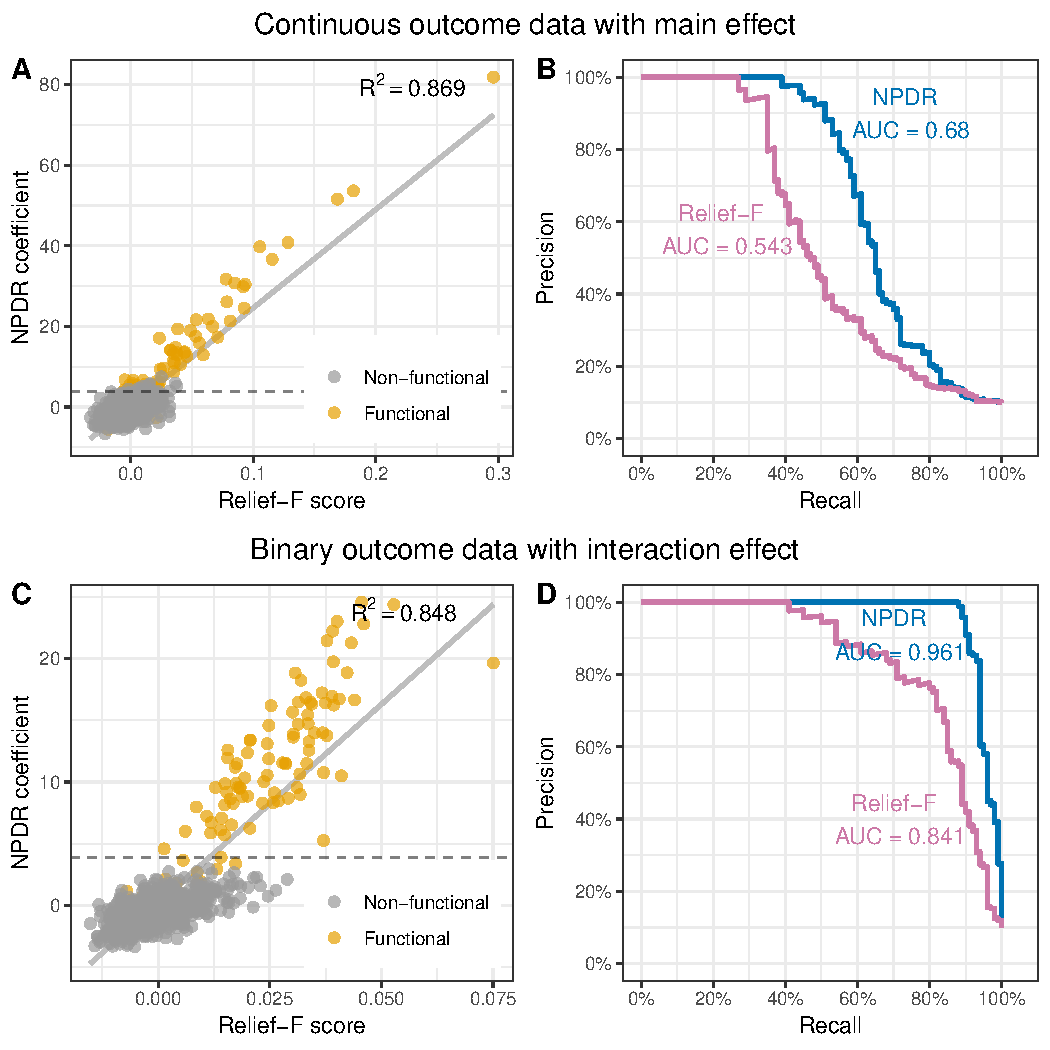
\includegraphics[trim = 0 0 0 0]{../figs/fig1.pdf}}
\caption{{\bf Comparison of NPDR and Relief-F results} for continuous outcome data with main effect (A-B) and binary outcome data with interaction effect (C-D). Importance score computed from the Relief-F and NPDR algorithm (standardized $\beta$ coefficient, Table \ref{tab:compare_npdr}) from one replicate of simulation with $m = 200$ samples and $p = 1000$ attributes (A, C). Area under the precision-recall curve used to assess algorithm performance (B, D).}
\label{fig:npdr_relief}
\end{figure}

For a dataset of the size simulated in our study ($m=200$ samples and $p=1000$ attributes), NPDR has a [X]-second runtime on a desktop with an Intel Xeon W-2104 CPU and 32GB of RAM. 

% Old: The increasing Recall with $k$ is expected for main effects because ReliefF becomes more myopic (more like a univariate t-test) as $k$ increases \cite{robnik03,mckinney13}. The increase in Recall is limited in part by the maximum number of neighbors being $\bar{k}_{\max{}} =\lfloor (m-1)/2\rfloor=49$. 

\subsection{Simulation comparison for continuous outcome data} 
For simulated data with continuous outcomes, we compare NPDR using a linear model (Eq.~\ref{eq:lin_reg}) with standard RReliefF from CORElearn, [and univariate linear regression].
Because CORElearn does not include the adaptive multiSURF neighborhood, we use a fixed-$k$ neighborhood $\mathcal{N}_{\bar{k}_{1/2}}$ for NPDR and RReliefF.
The [value] $\bar{k}_{1/2}=30$ (Eq.~\ref{eq:kbar}) is the expected number of nearest neighbors corresponding to a multiSURF neighborhood.
Because of the structural difference between simulation of main and interaction effect, it is not trivial to 
Therefore, we aim to simulate similar correlation between NPDR and Relief-F importance score as in the case of binary outcome data with interaction effect (Fig. \ref{fig:npdr_relief}C).
The auPRC of both methods are less than before, which is likely due to differences in the simulated effect size as well as underlying structure of the data.
Nevertheless, across 100 simulations, NPDR still yields significantly higher auPRC (P < 0.0001, see Supplementary Fig. S3).


% \begin{figure}[h]
% \centerline{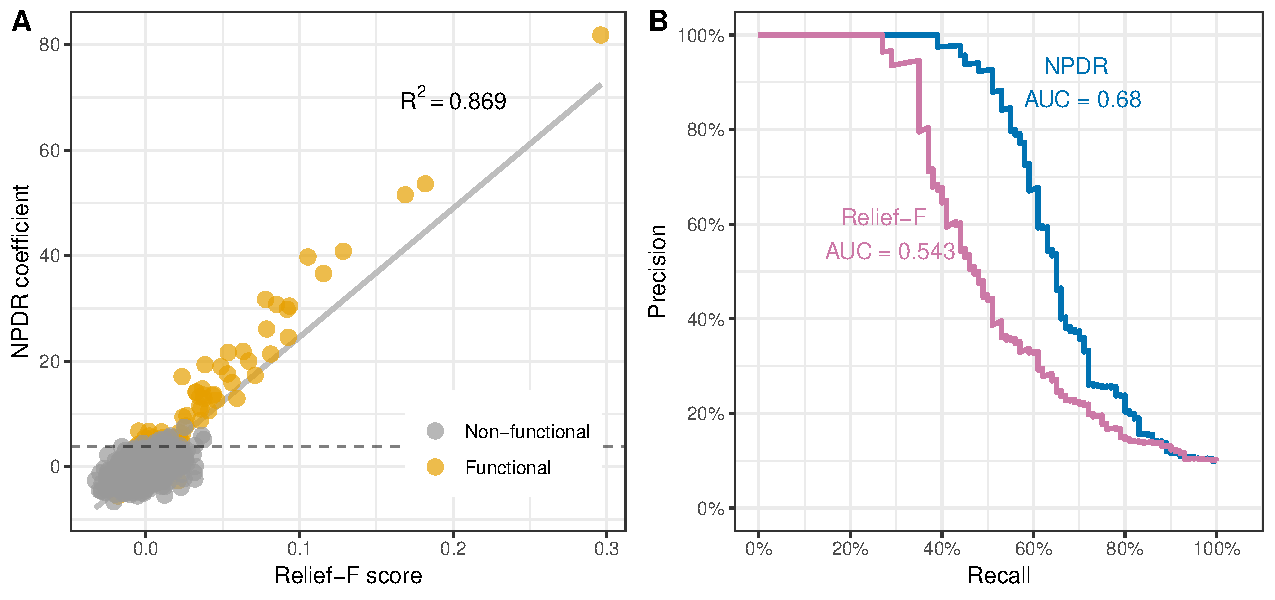
\includegraphics[]{../figs/npdr_relief_qtrait.pdf}}
% \caption{{\bf Comparison of NPDR and Relief-F results for continuous outcome data.} Importance score computed from the Relief-F and NPDR algorithm (standardized $\beta$ coefficient, Table \ref{tab:compare_npdr}) from one replicate of simulation with $m = 100$ samples and $p = 100$ attributes (A). Area under the precision-recall curve used to assess algorithm performance (B).}
% \label{fig:npdr_relief_qtrait}
% \end{figure}

\subsection{Real-world RNA-Seq data with confounding}

TODO:
- Also show univariate analysis with and without adjustment in supplement? 


With multiSURF neighborhood $\mathcal{N}_{\alpha=1/2}$, we apply NPDR with and without adjusting for the sex covariate.
Several genes including UTY, PRKY, and USP9Y are removed from the list of MDD-associated genes when you adjust for the sex covariate, which indicates suprious associations between these genes and diagnostic phenotype due to confounding by sex.
These genes are Y-linked (i.e., Y chromosome (male)) genes and mainly expressed in testis.
For example, the RPS4Y2 ribosomal protein S4 Y-linked 2 has been shown by tissue specific studies to mainly express in prostate and testis \cite{lopes2010human}.
Meanwhile, highly expressed in the brain as well as testis, the gene C2orf55 (KIAA1211L) is associated with sex but remains in the adjusted NPDR list ($p_\textrm{adj} < 0.05$) and may be relevant to MDD pathophysiology.
[other genes here]
In summary, this comparison suggests the NPDR with covariate adjustment effectively removes sex-related confounding variables.
A list of 485 genes with expression associated with sex (Bonferroni-adjusted P value $<0.0001$) and their statistical significance are included in the Supplementary Table S1.

\begin{figure}[!tpb]%figure2
\centerline{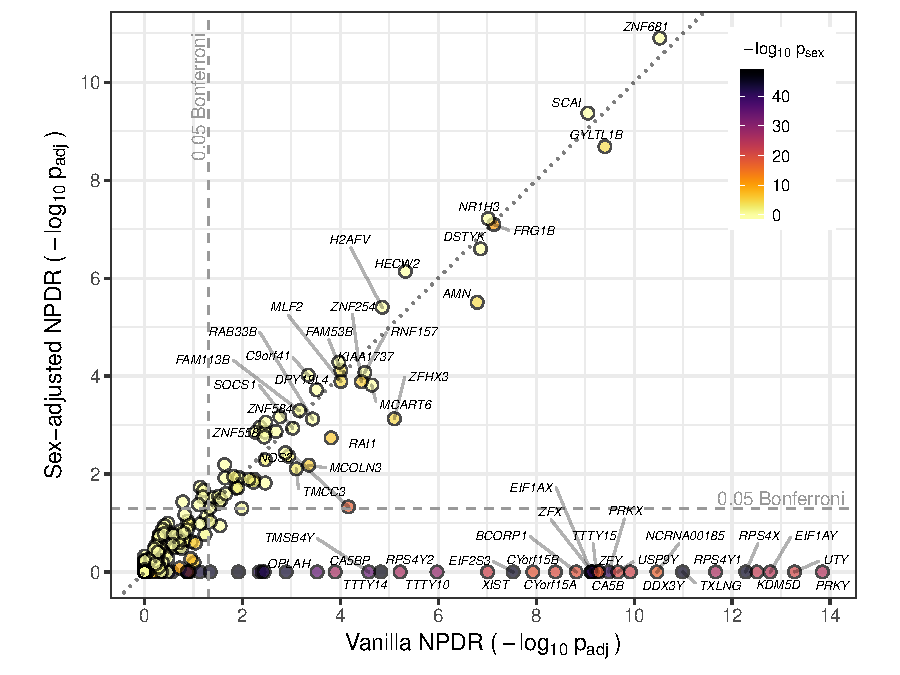
\includegraphics[]{../figs/mostafavi_npdrs_mdd.pdf}}
\caption{{\bf To adjust or not to adjust.}
Gene scatter plot of $-\log_{10}$ adjusted significance for association with major depressive disorder using NPDR without correction for sex (horizontal axis) and with correction for sex (vertical axis). NPDR without sex correction finds [47] genes that are significant at the Bonferroni-adjusted 0.05 level (above horizontal dashed line) [28] of which are also significantly associated with sex ($p^\textrm{sex}_\textrm{adj} < 0.05$).  NPDR with adjustment for sex finds [23] genes that are significant at the Bonferroni-adjusted 0.05 level (right of vertical dashed line) only 3 of which are also significantly associated with sex, thus eliminating most of the confounding variables.}
\label{fig:npdrs_mdd}
\end{figure}


Sensitivity to confounders extends beyond nearest-neighbors feature selection algorithms.
When covariates are not accounted for, even powerful methods are expected to produce biased attribute importance scores.
On the other hand, it is not trivial to include covariates in most widely used machine learning models including random forest.
Specifically, in random forest, only with the `ranger` `R` package do we have the option of always including the covariates (e.g., sex) in addition to a set number of random variables selected prior to node splitting.
However, this forced inclusion squashes the importance of other variables.
In the case of the current real RNASeq data analysis of MDD, when we utilized this option in `ranger`, the covariate ``sex" is more than 20 times more important than the next most important attriute (ZNF845).
The effect of forced inclusion of a particular covariate at node splitting on the entire algorithm is unclear.
More specific studies with simulations of covariates will prove useful in determining the effect of this implementation on the final result.


Moreover, like previous feature selection methods before STIR, importance scores produced by random forest does not follow a distribution.
Hence, instead of P values, we compare NPDR standardized $\beta$ coefficient and random forest Gini-based importance score (Fig. \ref{fig:npdr_rf_mdd}).
Most genes with high random forest importance score but low NPDR coefficient are highly associated with sex (dark pink - purple).
However, there is a consensus between the two methods in giving high scores for genes such as [].


\begin{figure}[!tpb]%figure2
\centerline{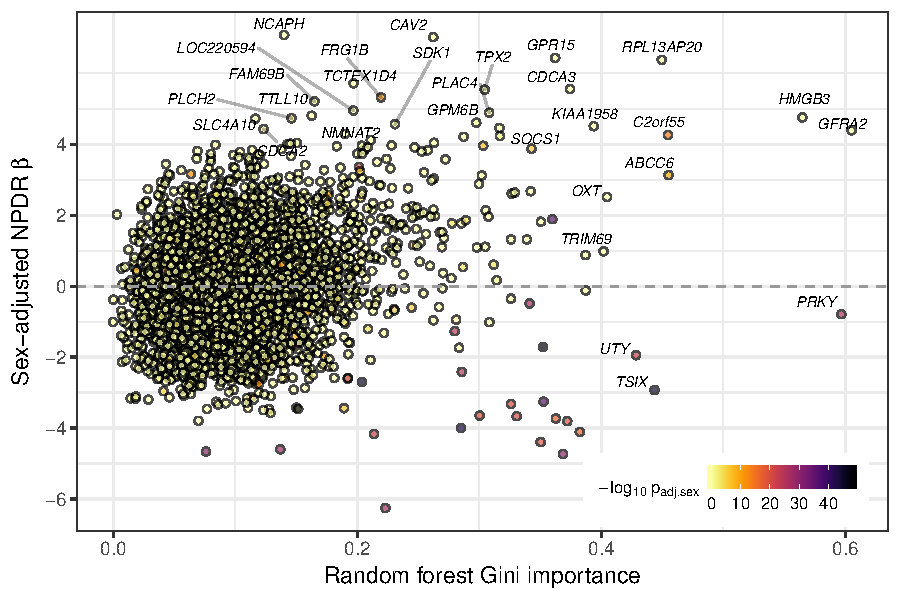
\includegraphics[]{../figs/npdr_rf_mdd.pdf}}
\caption{{\bf NPDR vs random forest feature importance.}
Gene scatter plot of importance score for association with major depressive disorder using random forest and NPDR with correction for sex. Many genes with high random forest importance score also have high association with sex. Genes are labeled if they are NPDR significance or have Gini importance $>0.4$.}
\label{fig:npdr_rf_mdd}
\end{figure}



%\textcolor{red}{Using STIR with fixed $k=m/6$, we identified 41 FDR-adjusted significant genes (not plotted). These 41 STIR $k=m/6$ genes include 31 of the 32 STIR-multiSURF genes. Thus, as we found in the simulation studies, these two versions of STIR perform similarly, with multiSURF being more conservative. Future studies will address the replication of the statistically significant STIR effects, the characterization of STIR interactions and the mathematical connection between neighbor-finding methods in STIR. The STIR runtime for the RNA-Seq data was approximately 19 seconds on a desktop with an Intel Xeon W-2104 CPU and 32GB of RAM. }
% Reproducing associations from the original study is not feasible because we focused on female subjects to avoid confounding (using 360 MDD and 282 controls) and Relief-based methods are currently not adept at correcting for covariates. However, we note that the top STIR association, Mitochondrial Pyruvate Carrier I (MPC1), also known as Brain Protein 44-Like (BRP44L), forms heterocomplex with MPC2 to mediate uptake of pyruvate into mitochondria (\cite{herzig12}). This interaction is noteworthy because MPC2 contains a variant that is associated with Schizophrenia in GWAS of East Asians (\cite{xiao16}). While an association with Schizophrenia seems indirect to MDD, symptom complexes such as anhedonia and psychosis can be shared across psychiatric disorders (\cite{lee13}).
% DSTYK, MIR324, HECW2, FBXL2, MDS2, RBPMS, PHKB, NHLH1, MED29, DMWD, PIBF1, APOBEC3C, NIPSNAP3A, MED19, OSBP2, PRG2, ADAMDEC1, ROR2, B4GALT7, GDPD3, BRP44L, LOC220594 and NELF.


 

%\citealp{Boffelli03} might want to know about  text text\break



\section{Discussion}
NPDR is the first method to our knowledge to combine projected distances and nearest-neighbors into a generalized linear model regression framework to perform feature selection. The use of nearest neighbors allows it to detect interacting attributes, an ability it shares with Relief-based methods, but NPDR is a departure from Relief in four ways. (1) For feature selection with a continuous outcome, it does not rely on the idea of a hit/miss group like current RRelief approaches~\cite{urbanowicz17}. Rather, NPDR simply does a regression between the outcome and attribute projected distances. (2) For feature selection with binary outcomes, NPDR uses a directional logistic model to fit pairwise projected distance regressors of hit and miss group. (3) This distance-based regression formalism provides a simple mechanism for NPDR to correct for covariates, which is often neglected in machine learning and has been a limitation of Relief-based methods. (4) For any outcome data type (binary or continuous) and predictor data type, NPDR computes the statistical significance of attribute importance scores, which allows for statistically based thresholds that can adjust for multiple hypothesis testing. (5) We introduced a regularized NPDR that adds another layer of multivariate modeling to an already multi-dimensional nearest-neighbor method to shrink correlated projected attribute differences.  

The regression formalism of NPDR is a novel way to perform RRelief by defining the attribute importance as the regression coefficient between the projected attribute differences and the numeric outcome differences between neighbors.  For linear regression, NPDR shares some similarity with the original RRelief algorithm because the regression coefficient is related to the correlation coefficient. The RRelief importance score is a weighted correlation between attribute and outcome differences, while the NPDR regression coefficient is a covariance between attribute and outcome differences divided by the variance in the outcome. The NPDR model may also include an offset if the diffs are not centered and the model may include correction terms for covariates that may be confounding. 

The original formulation of Relief was for binary outcome data, which lends itself naturally to nearest hit (same class) and miss (opposite class) neighbors. As discussed above, for regression problems, the original regression Relief (RRelief) score was cast as a weighted correlation between outcome and the attribute diff~\cite{robnik03}. In a different approach, Ref.~\cite{urbanowicz17} uses a standard deviation of the continuous outcome diffs to discretize the numeric outcome and make the RRelief algorithm compatible with the idea of hits and misses. However, discretization puts constraints on the variation in numeric data and has the risk of losing power. NPDR uses the full variation in the continuous outcome variable, and the regression coefficient provides an interpretation in terms of variation explained while again providing flexibility for modeling additional effects. 

We assessed NPDR's power and ability to control false positives using realistic simulations with main effects and network interactions. We showed that the statistical performance using NPDR p-values is the same as the original STIR, which is specific to binary outcome data. This indicates that NPDR, which models hit/miss differences between neighbors with a directional logit link, can be safely used instead of STIR with the added benefit of covariance correction and the analysis of quantitative traits. Comparison of NPDR for quantitative outcomes... 

We applied NPDR to a real RNA-Seq dataset for MDD to demonstrate the identification of biologically relevant genes and the removal of spurious associations by covariate correction. NPDR with sex as a covariate adjustment successfully removed X and Y linked genes and genes highly expressed in sex organs. It is important to note that some genes removed due to a shared association with sex may be important for the pathophysiology of MDD (C2orf55 (KIAA1211L)) or for classifiers.  Thus, covariate adjustment in NPDR is a useful option to inform a holistic analysis of a given dataset. Further improvements in the NPDR covariate adjustment may be achieved by correcting the distance matrix calculation. Adding a covariate term may not be sufficient in some cases because the neighborhood could be strongly influenced by confounding genes due to the curse of dimensionality. The curse of dimensionality can also affect confounding in distance matrix calculation.

%\subsection{Statistical Inference for Relief (STIR) with Subsampling Empirical Distribution}

%To regularize the effect of duplicates and obtain more conservative p-values, we propose a sampling approach $W_{STIR}$ in which we draw the hit and miss sets %($M$ and $H$) without replacement (subsample) $B$ times to create an empirical distribution of the $\myd$ sets 
%($M^*\subset M$ and $H^*\subset H$) for the t-test calculation. The sampled STIR weight is 
%\begin{equation}
%W_{STIR}[a,M,H]=W_{RT}[a,M^*,H^*]
%\end{equation}

%where the sampled set $M^*$ of nearest miss neighbors are drawn randomly without replacement $B[m,k_M]$ times (defined below) from the set M of size $m_{k_M}$. %In other words, miss neighbors $(\ri,\mji(\ri))$ are drawn from $M$, where $i=1,\dots, m$ and $j_i=1,\dots, \kmi$. Similarly, the hit set $H^*$ is obtained by %drawing $B[m,k_H]$ ordered hit pairs from $H$. Once the subset of hit and miss diffs is sampled, we compute the t-test as described above (Eqs. \ref{eq:stir}) %for all attributes and adjust the p-values for multiple testing.
%
%We use the following expression to compute the number of without-replacement samples B to perform on the hit and miss matrices
%\begin{equation}
%B[m,\ka]=\frac{m\ka}{2}\left(1+e^{1-\ka}\right),
%\end{equation}

%where the expression is parameterized by the number of instances, m, and the average number of neighbors in each hit/miss group $k_{\alpha=H}$ or %$k_{\alpha=M}$. The prefactor, $\frac{m\ka}{2}$, is the large-$\ka$ sampling limit to adjust for the number of redundant diffs that leads to an increased false %positive rate (the term in parentheses approaches 1). As $ka$ decreases, there is a decreased probability that a neighbor of instance $\ri$ also includes %$\ri$ in its neighborhood. When $\ka$ is small, there are fewer redundant neighbors and we wish to sample more of the available $m\ka$ diffs to increase the %power of the sampled t-test. When the average number of neighbors reaches its minimum, $\ka$=1, we use all $m\ka$ diffs. 

We also derived the theoretical mapping between the average $k$ expected for fixed-$k$ Relief neighborhoods and radius-based Relief neighborhoods. One reason this relationship is useful is to compare with implementations of Relief that do not include the multiSURF neighborhood. For fixed-$k$ neighborhoods, we expect the NPDR approach will handle imbalanced data in a less biased way than the original fixed-$k$ methods, which focus on hit/miss neighborhoods separately. By identifying the nearest neighbors independently of hit/miss status, the neighborhood should naturally reflect the imbalance in the data. The hit/miss status of each pair is computed separately as a categorical outcome regression variable. This should make NPDR scores with fixed-$k$ ($\mathcal{N}_{k_\alpha}$) similar to fixed radius ($\mathcal{N}_{R_\alpha}$) for balanced and imbalanced data.    

Power for detecting main effects is highest with the myopic maximum $k=k_{\text{max}}=\lfloor (m-1)/2\rfloor$. Real biological data will likely contain a mixture of main effects and epistasis network effects \cite{mckinney_pajewski}. STIR feature selection could be embedded in the backwards elimination of private Evaporative Cooling (privateEC) for feature selection and classification \cite{le17} or embedded in a nested cross-validation approach. Nested CV and privateEC can also return classification and optimize $\alpha$ or $k$. 

%The study focuses on obtaining a reasonable estimate of the probability of statistically significant association between an attribute and the outcome while taking into account the complex underlying architecture of interaction among attributes. 

Note to self. glmnet NPDR and using the $\text{d}^{\text{(type)}}_{ij}(A)$ design matrix of all attributes to create a $p \times p$ nearest-neighbor based gene network for hub and module based on the correlation between genes based on the projected distances vectors. Like STIR before it, NPDR P values suffer from deflation due to dependence among the nearest neighbors in the neighborhood, $\mathcal{N}$. The FDR procedure does a good job of selecting the true positives from the false positives (so I think it's not a really big concern), but it would be nice to address the dependence of neighbors in $\mathcal{N}$. One approach would be to create a batch-like indicator variable with $m$ states (a lot), indicating from which instance $i$ a batch of neighbors comes from. This neighbor batch could be used as a covariate in NPDR. Really case and controls should be evenly distributed within each ``batch,'' so I'm not sure this would solve the problem. Another thought is to create a weight variable that counts how often each pair happens and use this as a covariate. Another possible approach would be to use principle components of the design matrix (might require fixed-$k$) as covariates in the NPDR regression model. The hypothesis is that the PCs would capture the neighborhood structure within $\mathcal{N}$. Requires some thought on how to map down to PCs with $m$ samples from all the neighbor pairs.

A related distance-based regression method is Multivariate Distance Matrix Regression (MDMR)~\cite{schork12}. The MDMR approach uses an F-statistic to test for the association of distance matrices between two sets of factors. The MDMR regression is performed for the distance matrix for all pairs of instances, not a subset of nearest neighbors, which makes it susceptible to missing interactions. Also MDMR focuses on sets of factors, whereas NPDR projects distances onto each attribute, allowing for hypothesis testing of individual attributes (i.e., perform feature selection). While NPDR uses the context of all attributes to compute nearest neighbors, it focuses on the projected regression of each attribute at a time and uses the nearest neighbors to allow for detection of interactions. The ability to remove imposters from the set of nearest neighbors illustrates the blessings of dimensionality for Relief-based methods, but this class of nearest-neighbor methods is still, of course, susceptible to the curses of dimensionality~\cite{CoD}. NPDR can also be used to compute the importance of sets of factors. The penalized version of NPDR uses the set of all attributes in a multiple projected-distance regression.

Multi-state categorical outcomes can be analyzed (similar to multi-state ReliefF) with NPDR by grouping all miss types together. This can be improved by using multinomial regression in NPDR. Application to GWAS data requires no additional modifications of the algorithm other than specification of a different diff function for categorical variables~\cite{titv}, and the covariate option allows for principle components to be included to adjust for population structure. 

\section*{Acknowledgements}

\section*{Funding}
This work was supported in part by the National Institute of Health Grant Nos. GM121312 and GM103456 (to BAM). 

%This work has been supported by the... Text Text  Text Text.\vspace*{-12pt}

%\bibliographystyle{plain}
\bibliographystyle{unsrt}
\bibliography{NPDR_refs}   % name of bib file

\end{document}
